\documentclass[]{article}
\usepackage{lmodern}
\usepackage{amssymb,amsmath}
\usepackage{ifxetex,ifluatex}
\usepackage{fixltx2e} % provides \textsubscript
\ifnum 0\ifxetex 1\fi\ifluatex 1\fi=0 % if pdftex
  \usepackage[T1]{fontenc}
  \usepackage[utf8]{inputenc}
\else % if luatex or xelatex
  \ifxetex
    \usepackage{mathspec}
  \else
    \usepackage{fontspec}
  \fi
  \defaultfontfeatures{Ligatures=TeX,Scale=MatchLowercase}
\fi
% use upquote if available, for straight quotes in verbatim environments
\IfFileExists{upquote.sty}{\usepackage{upquote}}{}
% use microtype if available
\IfFileExists{microtype.sty}{%
\usepackage{microtype}
\UseMicrotypeSet[protrusion]{basicmath} % disable protrusion for tt fonts
}{}
\usepackage[margin=1in]{geometry}
\usepackage{hyperref}
\hypersetup{unicode=true,
            pdftitle={Trabalho de Estatística Aplicada},
            pdfauthor={Daniel dos Santos e Gabriel Mizuno},
            pdfborder={0 0 0},
            breaklinks=true}
\urlstyle{same}  % don't use monospace font for urls
\usepackage{graphicx,grffile}
\makeatletter
\def\maxwidth{\ifdim\Gin@nat@width>\linewidth\linewidth\else\Gin@nat@width\fi}
\def\maxheight{\ifdim\Gin@nat@height>\textheight\textheight\else\Gin@nat@height\fi}
\makeatother
% Scale images if necessary, so that they will not overflow the page
% margins by default, and it is still possible to overwrite the defaults
% using explicit options in \includegraphics[width, height, ...]{}
\setkeys{Gin}{width=\maxwidth,height=\maxheight,keepaspectratio}
\IfFileExists{parskip.sty}{%
\usepackage{parskip}
}{% else
\setlength{\parindent}{0pt}
\setlength{\parskip}{6pt plus 2pt minus 1pt}
}
\setlength{\emergencystretch}{3em}  % prevent overfull lines
\providecommand{\tightlist}{%
  \setlength{\itemsep}{0pt}\setlength{\parskip}{0pt}}
\setcounter{secnumdepth}{0}
% Redefines (sub)paragraphs to behave more like sections
\ifx\paragraph\undefined\else
\let\oldparagraph\paragraph
\renewcommand{\paragraph}[1]{\oldparagraph{#1}\mbox{}}
\fi
\ifx\subparagraph\undefined\else
\let\oldsubparagraph\subparagraph
\renewcommand{\subparagraph}[1]{\oldsubparagraph{#1}\mbox{}}
\fi

%%% Use protect on footnotes to avoid problems with footnotes in titles
\let\rmarkdownfootnote\footnote%
\def\footnote{\protect\rmarkdownfootnote}

%%% Change title format to be more compact
\usepackage{titling}

% Create subtitle command for use in maketitle
\newcommand{\subtitle}[1]{
  \posttitle{
    \begin{center}\large#1\end{center}
    }
}

\setlength{\droptitle}{-2em}

  \title{Trabalho de Estatística Aplicada}
    \pretitle{\vspace{\droptitle}\centering\huge}
  \posttitle{\par}
    \author{Daniel dos Santos e Gabriel Mizuno}
    \preauthor{\centering\large\emph}
  \postauthor{\par}
      \predate{\centering\large\emph}
  \postdate{\par}
    \date{04 de Setembro de 2018}

\usepackage{booktabs} \usepackage{longtable} \usepackage{array}
\usepackage{multirow} \usepackage[table]{xcolor} \usepackage{wrapfig}
\usepackage{float} \floatplacement{figure}{H} \usepackage{booktabs}
\usepackage{multirow} \usepackage{rotating} \usepackage{indentfirst}

\begin{document}
\maketitle

{
\setcounter{tocdepth}{3}
\tableofcontents
}
\subsection{1-) Objetivo:}\label{objetivo}

\begin{itemize}
\tightlist
\item
  Montar um perfil dos clientes segundo seu sexo.\\
\item
  Avalar o perfil dos clientes co conta bancária em relação à satisfação
  com o limite de crédito desponível.
\end{itemize}

\subsection{2-) Metodologia:}\label{metodologia}

Foi realizados os seguintes testes para responder os objetivos desse
relatório Qui-Quadrado, Teste de Hipóteses para Média, Teste de
Hipóteses para Variância e Teste de Kolmogorov-Smirnov usando um nível
de significância de 10\% (\(\alpha\)=10\%). Para a análise e confecção
desse relatório foram avaliadas somente algumas variáveis que foram
consideradas de interesse para responder as perguntas 1 e 2.

\subsection{3-) Análise dos Resultados:}\label{analise-dos-resultados}

Com base nos resultados da base de dados, no nível de significância
(estabelecido na seção anterior) e usando os testes e análises
descritivas adequados, para cada situação, podemos concluímos para o
\textbf{1º objetivo} que:

\begin{itemize}
\tightlist
\item
  Utilizando o teste Qui-Quadrado podemos dizer que as variáveis
  ``Banco'' e ``Satisfeito com o limite'' são independentes (usando o
  p-valor da tabela \ref{table:tab1}).
\item
  Primeiro temos que pelo teste de Kolmogorov-Smirnov que as amostras
  possuem distribuição normal para o nível de significância de 10\%,
  temos também que pelo t-test que a média de idade das pessoas não
  satisfeitas com o limite oferecido é maior do as que estão satisfeitas
  com seu limite (p-valor=0.1445\textgreater{}\(\alpha\)).
\item
  Utilizando o teste Qui-Quadrado podemos dizer que as variáveis
  ``Banco'' e ``Satisfeito com o limite'' são independentes (usando o
  p-valor da tabela \ref{table:tab1}).
\end{itemize}

\textbf{2º objetivo:}

\begin{itemize}
\tightlist
\item
  Para analisarmos as variáveis ``Tempo que é cliente'' e ``Satisfeito
  com o limite'' estamos considerando que temos normalidade assintótica,
  nesse cenário podemos dizer que a média de idade de quem é satisfeito
  com o limite é maior do quem não é satisfeito
  (p-valor=0.01669\textless{}\(\alpha\)).
\item
  Utilizando o teste Qui-Quadrado podemos dizer que as variáveis ``Falou
  com gerente'' e ``Satisfeito com o limite'' são independentes (usando
  o p-valor da tabela \ref{table:tab1}).
\item
  Utilizando o teste Qui-Quadrado podemos dizer que as variáveis
  ``sexo'' e ``Satisfeito com o limite'' são dependentes (usando o
  p-valor da tabela \ref{table:tab1}).
\end{itemize}

\pagebreak

\subsection{4-) Conclusão:}\label{conclusao}

Verificamos, seção anterior, que há uma relação entre as variáveis
``sexo'' e ``possuir nome no SERASA'', utilizando a analise descritiva
na \ref{table:tab2} temos evidências que dos possuem nome no SERASA a
maioria (64.9\%) são homens já as mulheres estão em minoria com 35.1\%.
Por outro lado, os homens são os mais satisfeitos com o limite da conta,
acreditamos que o limite oferecido aos homens é incompatível com a
situação de inadimplência. Sendo assim, seria mais adequado reduzir o
limite dos homens e oferecer para a mulher não inadimplentes um limite
maior.

Pensando quanto a satisfação dos clientes em relação limite oferecido
podemos afirmar que os clientes do Bradesco são proporcionalmente mais
satisfeitos com limite oferecido (80\%), já a Caixa possui a maior
porcentagem de insatisfação dos clientes com o limite.

Usando os teste adequado, a tabela \ref{table:tab2} e um boxplot gráfico
,presente no apêndice, podemos dizer que o tempo de uso semanal do
Bankline aumentou para quem fez o curso. Portanto, suspeitamos que o
curso incentivou o usuário usar mais os serviço disponíveis no Bankline
sendo assim o curso foi efetivo.

\pagebreak 

\subsection{5-)Apêndice:}\label{apendice}

\subsubsection{5.1-) Figuras:}\label{figuras}

\begin{figure}
\centering
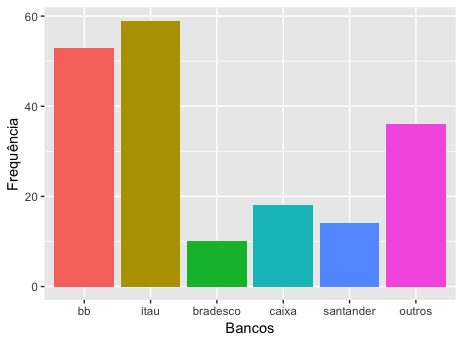
\includegraphics[width=3.12500in]{Bancos.png}
\caption{Número de clientes por banco}
\end{figure}

\begin{figure}
\centering
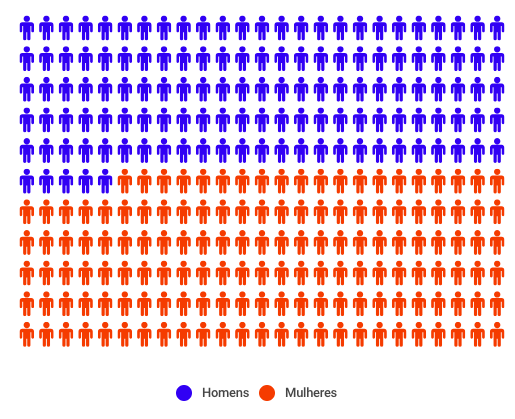
\includegraphics[width=3.12500in]{pictograma.png}
\caption{Quantidade de mulheres e homens}
\end{figure}

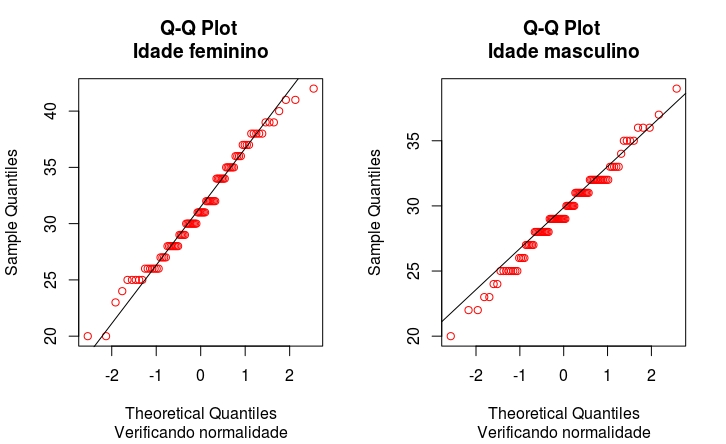
\includegraphics[width=3.12500in]{QQ Plot idade genero.jpeg}
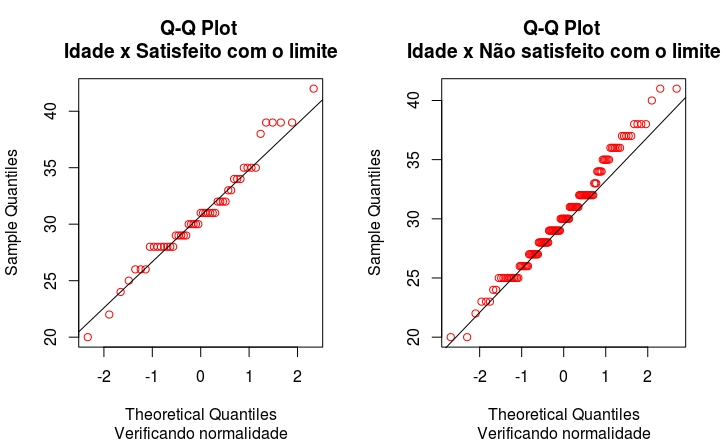
\includegraphics[width=3.12500in]{QQplot Idade x Lim.jpeg}

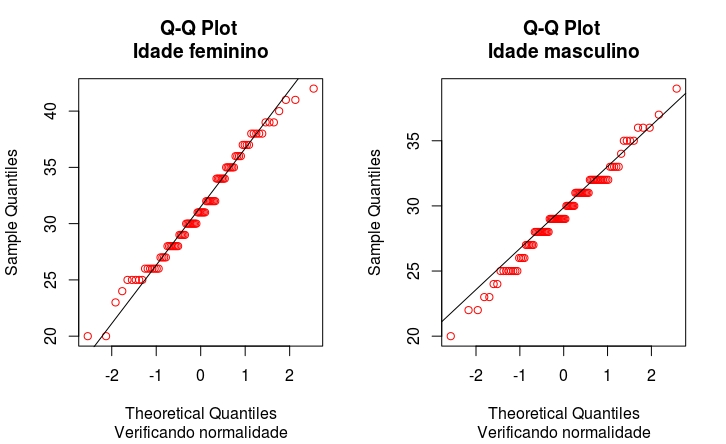
\includegraphics[width=3.12500in]{QQ Plot idade genero.jpeg}
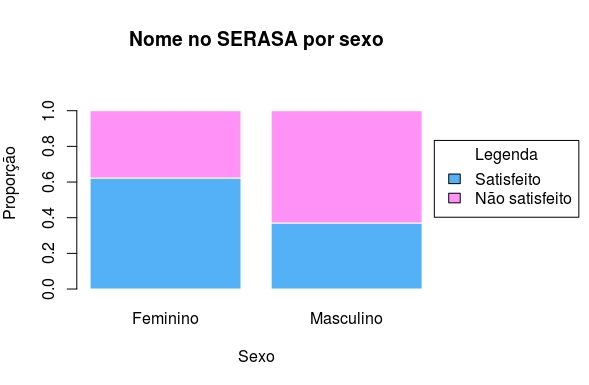
\includegraphics[width=3.12500in]{Nome no SERASA por sexo.jpeg}

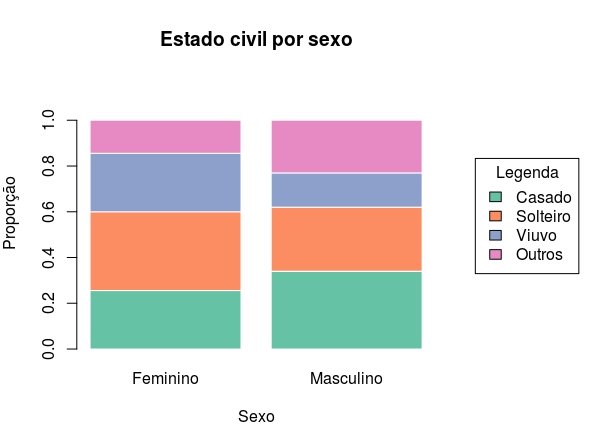
\includegraphics[width=3.12500in]{Estado civil por Sexo.jpeg}
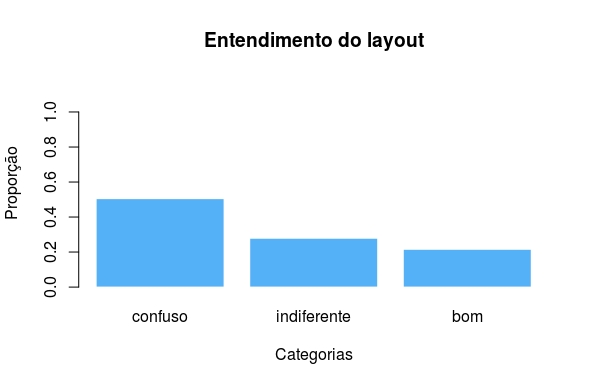
\includegraphics[width=3.12500in]{Entedimento do Layout.jpeg}

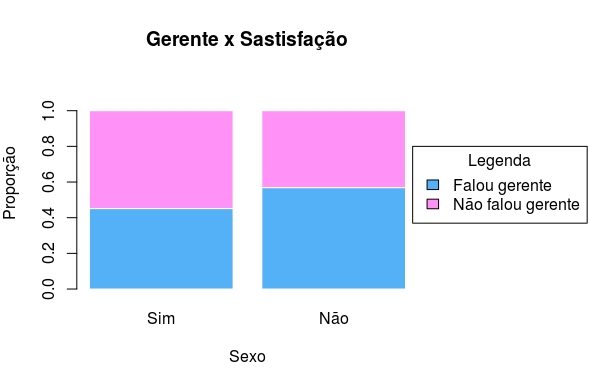
\includegraphics[width=3.12500in]{Gerente Satisfacao.jpeg}
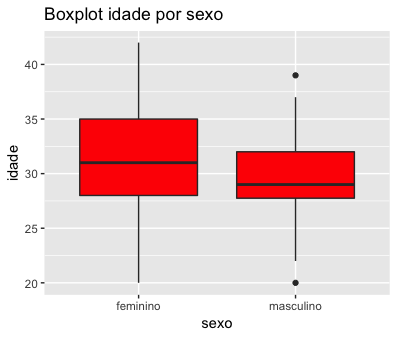
\includegraphics[width=3.12500in]{boxplot_idade_genero.png}
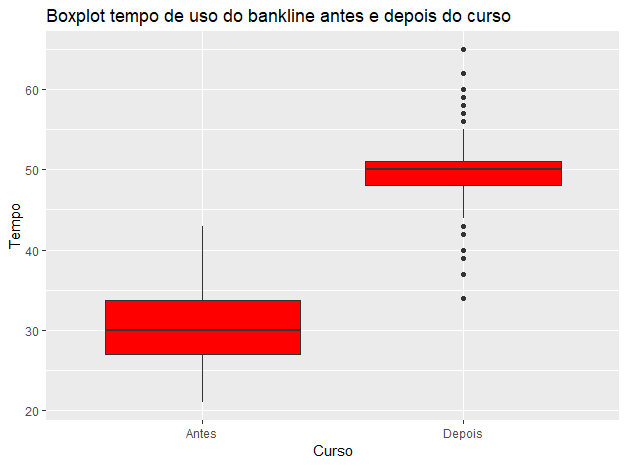
\includegraphics[width=3.12500in]{Tempo e Curso.png}
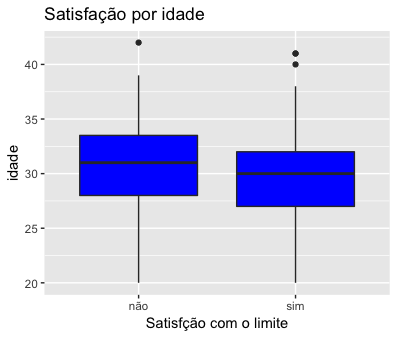
\includegraphics[width=3.12500in]{idade_satis.png} \pagebreak 

\subsubsection{5.2-) Tabelas:}\label{tabelas}

\begin{table*}[h!]
    \centering
        \caption{Tabela de contigência com p-valor}
        \begin{tabular}{c c c c c c c c c}
            \toprule
            \midrule
                & & \multicolumn{4}{c}{Sexo}\\ \cmidrule{3-9}
                && \multicolumn{2}{c}{Masculino} & \multicolumn{2}{c}{Feminino} & \multicolumn{2}{c}{Total} \\ \cmidrule{3-9}
                && n & \% & n & \% & n & \% & P-Valor \\ \cmidrule{3-9}
                \multicolumn{1}{c}{\multirow{5}{*}}   &
                \multicolumn{1}{l}{\textbf{SERASA}} &  &  &  & & &  & \textcolor{red}{0.0005155} \\ \cmidrule{1-9}
                \multicolumn{1}{c}{}    &
                \multicolumn{1}{l}{Não} & 37 & 39.8 & 56 & 60.2 & 93 & 48.9 &  \\
                \multicolumn{1}{c}{}    &
                \multicolumn{1}{l}{Sim}& 63 & 64.9 & 34 & 35.1 & 97 & 51.1  \\ \cmidrule{1-9} &
                \multicolumn{1}{l}{\textbf{Estado Civil}} &  &  &  & & &  & 0.1882 \\ \cmidrule{1-9}                
                \multicolumn{1}{c}{}    &
                \multicolumn{1}{l}{Casado} & 34 & 40.4 & 23 & 59.6 & 57 & 30 &  \\
                \multicolumn{1}{c}{}    &   
                \multicolumn{1}{l}{Solteiro} & 28 & 52.5 & 31 & 47.5 & 59 & 31.1 &  \\
                \multicolumn{1}{c}{}    &
                \multicolumn{1}{l}{Viúvo} & 15 & 60.5 & 23 & 39.5 & 38 & 20   \\
                \multicolumn{1}{c}{}    &
                \multicolumn{1}{l}{Outros} & 23 & 36.1 & 13 & 63.9& 36 & 18.9   \\  
                \toprule
                \midrule 
                & & \multicolumn{4}{c}{Satisfeito com limite}\\ \cmidrule{3-9}
                && \multicolumn{2}{c}{Não} & \multicolumn{2}{c}{Sim} & \multicolumn{2}{c}{Total}  \\ \cmidrule{3-9}
                && n & \% & n & \% & n & \% & P-Valor \\ \cmidrule{3-9}
                \multicolumn{1}{c}{\multirow{5}{*}}   &
                \multicolumn{1}{l}{\textbf{SERASA}} &  &  &  & & &  & 0.5203 \\ \cmidrule{1-9}
                \multicolumn{1}{c}{}    &
                \multicolumn{1}{l}{Não} & 23 & 24.7 & 70 & 75.3 & 93 & 48.9 &  \\
                \multicolumn{1}{c}{}    &
                \multicolumn{1}{l}{Sim}& 28 & 28.9 & 69 & 71.1 & 97 & 51.1 \\ \cmidrule{1-9} &
                \multicolumn{1}{l}{\textbf{Banco}}&  &  &  & & &  & 0.1366\\ \cmidrule{1-9}                
                \multicolumn{1}{c}{}    &
                \multicolumn{1}{l}{BB} & 17 & 32.1 & 36 & 67.9 & 53 & 27.9  \\
                \multicolumn{1}{c}{}    &   
                \multicolumn{1}{l}{Itaú} &16 & 27.1 & 43 & 72.9 & 59 & 31.1  \\
                \multicolumn{1}{c}{}    &
                \multicolumn{1}{l}{Bradesco} & 2 & 20 & 8 & 80 & 10 & 5.3 \\
                \multicolumn{1}{c}{}    &
                \multicolumn{1}{l}{Caixa} & 8 & 44.1 & 10 & 55.9 & 36 & 18.9  \\
                \multicolumn{1}{c}{}    &
                \multicolumn{1}{l}{Santander} & 4 & 28.6 & 10 & 71.4 & 14 & 7.4  \\
                \multicolumn{1}{c}{}    &
                \multicolumn{1}{l}{Outros} & 4 & 11.1 & 32 & 88.9  & 36 & 18.9\\ \cmidrule{1-9} &
                \multicolumn{1}{l}{\textbf{Gerente}} &   &  &  & & &  & 0.1505 \\ \cmidrule{1-9}
                \multicolumn{1}{c}{}    &
                \multicolumn{1}{l}{Não} & 28 & 31.8 & 60 & 68.2 & 88 & 48.9 &  \\
                \multicolumn{1}{c}{}    &
                \multicolumn{1}{l}{Sim}& 23 & 22.5 & 79 & 77.5 & 102 & 51.1  \\ \cmidrule{1-9} &
                \multicolumn{1}{l}{\textbf{Sexo}} &   &  &  & & &  & \textcolor{red}{0.001251} \\ \cmidrule{1-9}
                \multicolumn{1}{c}{}    &
                \multicolumn{1}{l}{Feminino} & 34 & 37.8 & 56 & 62.2 & 90 & 47.4 &  \\
                \multicolumn{1}{c}{}    &
                \multicolumn{1}{l}{Masculino}& 17 & 17 & 79 & 83 & 83 & 52.6  \\
                \midrule
                \bottomrule
        \end{tabular}
        \centering
        \label{table:tab1}
        \label{tab:sam_count}
\end{table*}

\begin{table}[h!]
  \begin{center}
  \caption{Tabela com algumas medidas resumo}
    \begin{tabular}{c|c|c|c|c|c|c|c}
    \hline
      \textbf{Variável} & \textbf{Min} & \textbf{Max} & \textbf{1º Q} & \textbf{2º Q} & \textbf{3º Q} & \textbf{Média}  & \textbf{Desvio Padrão} \\
      \hline
      Idade & 20 & 42 & 28 & 30 & 32.75 & 30.37 & 4.3\\
      Tempo de uso do Bankline antes do curso & 21 & 43 & 27 & 30 & 33.75 & 30.28 & 4.53\\
      Tempo de uso do Bankline depois do curso & 34 & 65 & 48 & 50 & 51 & 49.92 & 3.87 \\ 
      \hline
    \end{tabular}
     \label{table:tab2}
  \end{center}
\end{table}


\end{document}
